
%% bare_jrnl.tex
%% V1.3
%% 2007/01/11
%% by Michael Shell
%% see http://www.michaelshell.org/
%% for current contact information.
%%
%% This is a skeleton file demonstrating the use of IEEEtran.cls
%% (requires IEEEtran.cls version 1.7 or later) with an IEEE journal paper.
%%
%% Support sites:
%% http://www.michaelshell.org/tex/ieeetran/
%% http://www.ctan.org/tex-archive/macros/latex/contrib/IEEEtran/
%% and
%% http://www.ieee.org/



% *** Authors should verify (and, if needed, correct) their LaTeX system  ***
% *** with the testflow diagnostic prior to trusting their LaTeX platform ***
% *** with production work. IEEE's font choices can trigger bugs that do  ***
% *** not appear when using other class files.                            ***
% The testflow support page is at:
% http://www.michaelshell.org/tex/testflow/


%%*************************************************************************
%% Legal Notice:
%% This code is offered as-is without any warranty either expressed or
%% implied; without even the implied warranty of MERCHANTABILITY or
%% FITNESS FOR A PARTICULAR PURPOSE! 
%% User assumes all risk.
%% In no event shall IEEE or any contributor to this code be liable for
%% any damages or losses, including, but not limited to, incidental,
%% consequential, or any other damages, resulting from the use or misuse
%% of any information contained here.
%%
%% All comments are the opinions of their respective authors and are not
%% necessarily endorsed by the IEEE.
%%
%% This work is distributed under the LaTeX Project Public License (LPPL)
%% ( http://www.latex-project.org/ ) version 1.3, and may be freely used,
%% distributed and modified. A copy of the LPPL, version 1.3, is included
%% in the base LaTeX documentation of all distributions of LaTeX released
%% 2003/12/01 or later.
%% Retain all contribution notices and credits.
%% ** Modified files should be clearly indicated as such, including  **
%% ** renaming them and changing author support contact information. **
%%
%% File list of work: IEEEtran.cls, IEEEtran_HOWTO.pdf, bare_adv.tex,
%%                    bare_conf.tex, bare_jrnl.tex, bare_jrnl_compsoc.tex
%%*************************************************************************

% Note that the a4paper option is mainly intended so that authors in
% countries using A4 can easily print to A4 and see how their papers will
% look in print - the typesetting of the document will not typically be
% affected with changes in paper size (but the bottom and side margins will).
% Use the testflow package mentioned above to verify correct handling of
% both paper sizes by the user's LaTeX system.
%
% Also note that the "draftcls" or "draftclsnofoot", not "draft", option
% should be used if it is desired that the figures are to be displayed in
% draft mode.



 % TO DELETE

    \documentclass[journal,a4paper]{IEEEtran}
 %    \documentclass[10pt,twocolumn,twoside]{IEEEtran}
%     \documentclass[11pt,draftcls,onecolumn,peerreview]{IEEEtran} 
%         \topmargin       -6.0mm
%          \oddsidemargin      0mm
%          \evensidemargin     0mm
%          \textheight     223.5mm
%         \textwidth      170.0mm

\usepackage{color}
\newcommand{\mike}[1]{\textsf{\emph{\textbf{\textcolor{red}{#1}}}}} 
\newcommand{\dean}[1]{\textsf{\emph{\textbf{\textcolor{green}{#1}}}}} 
\newcommand{\parham}[1]{\textsf{\emph{\textbf{\textcolor{blue}{#1}}}}} 
\newcommand{\ken}[1]{\textsf{\emph{\textbf{\textcolor{magenta}{#1}}}}} 
\newcommand{\cut}[1]{\textcolor{cyan}{#1}} 



% If IEEEtran.cls has not been installed into the LaTeX system files,
% manually specify the path to it like:
% \documentclass[journal]{../sty/IEEEtran}





% Some very useful LaTeX packages include:
% (uncomment the ones you want to load)


% *** MISC UTILITY PACKAGES ***
%
%\usepackage{ifpdf}
% Heiko Oberdiek's ifpdf.sty is very useful if you need conditional
% compilation based on whether the output is pdf or dvi.
% usage:
% \ifpdf
%   % pdf code
% \else
%   % dvi code
% \fi
% The latest version of ifpdf.sty can be obtained from:
% http://www.ctan.org/tex-archive/macros/latex/contrib/oberdiek/
% Also, note that IEEEtran.cls V1.7 and later provides a builtin
% \ifCLASSINFOpdf conditional that works the same way.
% When switching from latex to pdflatex and vice-versa, the compiler may
% have to be run twice to clear warning/error messages.






% *** CITATION PACKAGES ***
%
\usepackage{cite}
% cite.sty was written by Donald Arseneau
% V1.6 and later of IEEEtran pre-defines the format of the cite.sty package
% \cite{} output to follow that of IEEE. Loading the cite package will
% result in citation numbers being automatically sorted and properly
% "compressed/ranged". e.g., [1], [9], [2], [7], [5], [6] without using
% cite.sty will become [1], [2], [5]--[7], [9] using cite.sty. cite.sty's
% \cite will automatically add leading space, if needed. Use cite.sty's
% noadjust option (cite.sty V3.8 and later) if you want to turn this off.
% cite.sty is already installed on most LaTeX systems. Be sure and use
% version 4.0 (2003-05-27) and later if using hyperref.sty. cite.sty does
% not currently provide for hyperlinked citations.
% The latest version can be obtained at:
% http://www.ctan.org/tex-archive/macros/latex/contrib/cite/
% The documentation is contained in the cite.sty file itself.






% *** GRAPHICS RELATED PACKAGES ***
%
\ifCLASSINFOpdf
   \usepackage[pdftex]{graphicx}
  % declare the path(s) where your graphic files are
  % \graphicspath{{../pdf/}{../jpeg/}}
  % and their extensions so you won't have to specify these with
  % every instance of \includegraphics
  % \DeclareGraphicsExtensions{.pdf,.jpeg,.png}
\else
  % or other class option (dvipsone, dvipdf, if not using dvips). graphicx
  % will default to the driver specified in the system graphics.cfg if no
  % driver is specified.
  \usepackage[dvips]{graphicx}
  % declare the path(s) where your graphic files are
  % \graphicspath{{../eps/}}
  % and their extensions so you won't have to specify these with
  % every instance of \includegraphics
  % \DeclareGraphicsExtensions{.eps}
\fi
% graphicx was written by David Carlisle and Sebastian Rahtz. It is
% required if you want graphics, photos, etc. graphicx.sty is already
% installed on most LaTeX systems. The latest version and documentation can
% be obtained at: 
% http://www.ctan.org/tex-archive/macros/latex/required/graphics/
% Another good source of documentation is "Using Imported Graphics in
% LaTeX2e" by Keith Reckdahl which can be found as epslatex.ps or
% epslatex.pdf at: http://www.ctan.org/tex-archive/info/
%
% latex, and pdflatex in dvi mode, support graphics in encapsulated
% postscript (.eps) format. pdflatex in pdf mode supports graphics
% in .pdf, .jpeg, .png and .mps (metapost) formats. Users should ensure
% that all non-photo figures use a vector format (.eps, .pdf, .mps) and
% not a bitmapped formats (.jpeg, .png). IEEE frowns on bitmapped formats
% which can result in "jaggedy"/blurry rendering of lines and letters as
% well as large increases in file sizes.
%
% You can find documentation about the pdfTeX application at:
% http://www.tug.org/applications/pdftex





% *** MATH PACKAGES ***
%
\usepackage[cmex10]{amsmath}
\interdisplaylinepenalty=2500
% A popular package from the American Mathematical Society that provides
% many useful and powerful commands for dealing with mathematics. If using
% it, be sure to load this package with the cmex10 option to ensure that
% only type 1 fonts will utilized at all point sizes. Without this option,
% it is possible that some math symbols, particularly those within
% footnotes, will be rendered in bitmap form which will result in a
% document that can not be IEEE Xplore compliant!
%
% Also, note that the amsmath package sets \interdisplaylinepenalty to 10000
% thus preventing page breaks from occurring within multiline equations. Use:
%\interdisplaylinepenalty=2500
% after loading amsmath to restore such page breaks as IEEEtran.cls normally
% does. amsmath.sty is already installed on most LaTeX systems. The latest
% version and documentation can be obtained at:
% http://www.ctan.org/tex-archive/macros/latex/required/amslatex/math/
\usepackage{amssymb}




% *** SPECIALIZED LIST PACKAGES ***
%
%\usepackage{algorithmic}
% algorithmic.sty was written by Peter Williams and Rogerio Brito.
% This package provides an algorithmic environment fo describing algorithms.
% You can use the algorithmic environment in-text or within a figure
% environment to provide for a floating algorithm. Do NOT use the algorithm
% floating environment provided by algorithm.sty (by the same authors) or
% algorithm2e.sty (by Christophe Fiorio) as IEEE does not use dedicated
% algorithm float types and packages that provide these will not provide
% correct IEEE style captions. The latest version and documentation of
% algorithmic.sty can be obtained at:
% http://www.ctan.org/tex-archive/macros/latex/contrib/algorithms/
% There is also a support site at:
% http://algorithms.berlios.de/index.html
% Also of interest may be the (relatively newer and more customizable)
% algorithmicx.sty package by Szasz Janos:
% http://www.ctan.org/tex-archive/macros/latex/contrib/algorithmicx/




% *** ALIGNMENT PACKAGES ***
%
% \usepackage{array}
% Frank Mittelbach's and David Carlisle's array.sty patches and improves
% the standard LaTeX2e array and tabular environments to provide better
% appearance and additional user controls. As the default LaTeX2e 
% generation code is lacking to the point of almost being broken with
% respect to the quality of the end results, all users are strongly
% advised to use an enhanced (at the very least that provided by array.sty)
% set of table tools. array.sty is already installed on most systems. The
% latest version and documentation can be obtained at:
% http://www.ctan.org/tex-archive/macros/latex/required/tools/


%\usepackage{mdwmath}
%\usepackage{mdwtab}
% Also highly recommended is Mark Wooding's extremely powerful MDW tools,
% especially mdwmath.sty and mdwtab.sty which are used to format equations
% and tables, respectively. The MDWtools set is already installed on most
% LaTeX systems. The lastest version and documentation is available at:
% http://www.ctan.org/tex-archive/macros/latex/contrib/mdwtools/


% IEEEtran contains the IEEEeqnarray family of commands that can be used to
% generate multiline equations as well as matrices, tables, etc., of high
% quality.


%\usepackage{eqparbox}
% Also of notable interest is Scott Pakin's eqparbox package for creating
% (automatically sized) equal width boxes - aka "natural width parboxes".
% Available at:
% http://www.ctan.org/tex-archive/macros/latex/contrib/eqparbox/





% *** SUBFIGURE PACKAGES ***
% \usepackage[tight,footnotesize]{subfigure}
% subfigure.sty was written by Steven Douglas Cochran. This package makes it
% easy to put subfigures in your figures. e.g., "Figure 1a and 1b". For IEEE
% work, it is a good idea to load it with the tight package option to reduce
% the amount of white space around the subfigures. subfigure.sty is already
% installed on most LaTeX systems. The latest version and documentation can
% be obtained at:
% http://www.ctan.org/tex-archive/obsolete/macros/latex/contrib/subfigure/
% subfigure.sty has been superceeded by subfig.sty.
 \ifCLASSOPTIONcompsoc
  \usepackage[tight,normalsize,sf,SF]{subfigure}
\else
  \usepackage[tight,footnotesize]{subfigure}
\fi


%\usepackage[caption=false]{caption}
%\usepackage[font=footnotesize]{subfig}
% subfig.sty, also written by Steven Douglas Cochran, is the modern
% replacement for subfigure.sty. However, subfig.sty requires and
% automatically loads Axel Sommerfeldt's caption.sty which will override
% IEEEtran.cls handling of captions and this will result in nonIEEE style
% figure/table captions. To prevent this problem, be sure and preload
% caption.sty with its "caption=false" package option. This is will preserve
% IEEEtran.cls handing of captions. Version 1.3 (2005/06/28) and later 
% (recommended due to many improvements over 1.2) of subfig.sty supports
% the caption=false option directly:
%\usepackage[caption=false,font=footnotesize]{subfig}
%
% The latest version and documentation can be obtained at:
% http://www.ctan.org/tex-archive/macros/latex/contrib/subfig/
% The latest version and documentation of caption.sty can be obtained at:
% http://www.ctan.org/tex-archive/macros/latex/contrib/caption/




% *** FLOAT PACKAGES ***
%
%\usepackage{fixltx2e}
% fixltx2e, the successor to the earlier fix2col.sty, was written by
% Frank Mittelbach and David Carlisle. This package corrects a few problems
% in the LaTeX2e kernel, the most notable of which is that in current
% LaTeX2e releases, the ordering of single and double column floats is not
% guaranteed to be preserved. Thus, an unpatched LaTeX2e can allow a
% single column figure to be placed prior to an earlier double column
% figure. The latest version and documentation can be found at:
% http://www.ctan.org/tex-archive/macros/latex/base/



\usepackage{stfloats}
% stfloats.sty was written by Sigitas Tolusis. This package gives LaTeX2e
% the ability to do double column floats at the bottom of the page as well
% as the top. (e.g., "\begin{figure*}[!b]" is not normally possible in
% LaTeX2e). It also provides a command:
%\fnbelowfloat
% to enable the placement of footnotes below bottom floats (the standard
% LaTeX2e kernel puts them above bottom floats). This is an invasive package
% which rewrites many portions of the LaTeX2e float routines. It may not work
% with other packages that modify the LaTeX2e float routines. The latest
% version and documentation can be obtained at:
% http://www.ctan.org/tex-archive/macros/latex/contrib/sttools/
% Documentation is contained in the stfloats.sty comments as well as in the
% presfull.pdf file. Do not use the stfloats baselinefloat ability as IEEE
% does not allow \baselineskip to stretch. Authors submitting work to the
% IEEE should note that IEEE rarely uses double column equations and
% that authors should try to avoid such use. Do not be tempted to use the
% cuted.sty or midfloat.sty packages (also by Sigitas Tolusis) as IEEE does
% not format its papers in such ways.


%\ifCLASSOPTIONcaptionsoff
%  \usepackage[nomarkers]{endfloat}
% \let\MYoriglatexcaption\caption
% \renewcommand{\caption}[2][\relax]{\MYoriglatexcaption[#2]{#2}}
%\fi
% endfloat.sty was written by James Darrell McCauley and Jeff Goldberg.
% This package may be useful when used in conjunction with IEEEtran.cls'
% captionsoff option. Some IEEE journals/societies require that submissions
% have lists of figures/tables at the end of the paper and that
% figures/tables without any captions are placed on a page by themselves at
% the end of the document. If needed, the draftcls IEEEtran class option or
% \CLASSINPUTbaselinestretch interface can be used to increase the line
% spacing as well. Be sure and use the nomarkers option of endfloat to
% prevent endfloat from "marking" where the figures would have been placed
% in the text. The two hack lines of code above are a slight modification of
% that suggested by in the endfloat docs (section 8.3.1) to ensure that
% the full captions always appear in the list of figures/tables - even if
% the user used the short optional argument of \caption[]{}.
% IEEE papers do not typically make use of \caption[]'s optional argument,
% so this should not be an issue. A similar trick can be used to disable
% captions of packages such as subfig.sty that lack options to turn off
% the subcaptions:
% For subfig.sty:
% \let\MYorigsubfloat\subfloat
% \renewcommand{\subfloat}[2][\relax]{\MYorigsubfloat[]{#2}}
% For subfigure.sty:
% \let\MYorigsubfigure\subfigure
% \renewcommand{\subfigure}[2][\relax]{\MYorigsubfigure[]{#2}}
% However, the above trick will not work if both optional arguments of
% the \subfloat/subfig command are used. Furthermore, there needs to be a
% description of each subfigure *somewhere* and endfloat does not add
% subfigure captions to its list of figures. Thus, the best approach is to
% avoid the use of subfigure captions (many IEEE journals avoid them anyway)
% and instead reference/explain all the subfigures within the main caption.
% The latest version of endfloat.sty and its documentation can obtained at:
% http://www.ctan.org/tex-archive/macros/latex/contrib/endfloat/
%
% The IEEEtran \ifCLASSOPTIONcaptionsoff conditional can also be used
% later in the document, say, to conditionally put the References on a 
% page by themselves.





% *** PDF, URL AND HYPERLINK PACKAGES ***
%
%\usepackage{url}
% url.sty was written by Donald Arseneau. It provides better support for
% handling and breaking URLs. url.sty is already installed on most LaTeX
% systems. The latest version can be obtained at:
% http://www.ctan.org/tex-archive/macros/latex/contrib/misc/
% Read the url.sty source comments for usage information. Basically,
% \url{my_url_here}.





% *** Do not adjust lengths that control margins, column widths, etc. ***
% *** Do not use packages that alter fonts (such as pslatex).         ***
% There should be no need to do such things with IEEEtran.cls V1.6 and later.
% (Unless specifically asked to do so by the journal or conference you plan
% to submit to, of course. )


% correct bad hyphenation here
% \hyphenation{op-tical net-works semi-conduc-tor}
% Algorithms
\usepackage{float}
\floatstyle{ruled}
\newfloat{algorithm}{htbp}{loa}%[chapter]
\floatname{algorithm}{Algorithm}

\begin{document}
%
% paper title
% can use linebreaks \\ within to get better formatting as desired
\title{Multiresolution Neural Field Estimation }
%
%
% author names and IEEE memberships
% note positions of commas and nonbreaking spaces ( ~ ) LaTeX will not break
% a structure at a ~ so this keeps an author's name from being broken across
% two lines.
% use \thanks{} to gain access to the first footnote area
% a separate \thanks must be used for each paragraph as LaTeX2e's \thanks
% was not built to handle multiple paragraphs
%

\author{In no particular order: P. Aram, M. Dewar, D.R. Freestone, K.Scerri, D.B. Grayden and V. Kadirkamanathan % <-this % stops a space
\thanks{P. Aram* and V. Kadirkamanathan are with the Department of Automatic Control and Systems Engineering, University of Sheffield, Sheffield, S1 3JD, U.K. (e-mail:p.aram@sheffield.ac.uk; visakan@sheffield.ac.uk).}% <-this % stops a space
\thanks{M. Dewar is with the School of Informatics, University of Edinburgh, Edinburgh, EH8 9AB, U.K. (e-mail:mike.dewar@inf.ed.ac.uk)}}% <-this % stops a space
%\thanks{Manuscript received April 19, 2005; revised January 11, 2007.}}

% note the % following the last \IEEEmembership and also \thanks - 
% these prevent an unwanted space from occurring between the last author name
% and the end of the author line. i.e., if you had this:
% 
% \author{....lastname \thanks{...} \thanks{...} }
%                     ^------------^------------^----Do not want these spaces!
%
% a space would be appended to the last name and could cause every name on that
% line to be shifted left slightly. This is one of those "LaTeX things". For
% instance, "\textbf{A} \textbf{B}" will typeset as "A B" not "AB". To get
% "AB" then you have to do: "\textbf{A}\textbf{B}"
% \thanks is no different in this regard, so shield the last } of each \thanks
% that ends a line with a % and do not let a space in before the next \thanks.
% Spaces after \IEEEmembership other than the last one are OK (and needed) as
% you are supposed to have spaces between the names. For what it is worth,
% this is a minor point as most people would not even notice if the said evil
% space somehow managed to creep in.



% The paper headers
% \markboth{Journal of }%
% {Aram \MakeLowercase{\textit{et al.}}: Wavelet Multiresolution Spatio-Temporal Modelling Using the Integro-Difference Equation}
% The only time the second header will appear is for the odd numbered pages
% after the title page when using the twoside option.
% 
% *** Note that you probably will NOT want to include the author's ***
% *** name in the headers of peer review papers.                   ***
% You can use \ifCLASSOPTIONpeerreview for conditional compilation here if
% you desire.
 \ifCLASSOPTIONpeerreview
\else
\fi



% If you want to put a publisher's ID mark on the page you can do it like
% this:
%\IEEEpubid{0000--0000/00\$00.00~\copyright~2007 IEEE}
% Remember, if you use this you must call \IEEEpubidadjcol in the second
% column for its text to clear the IEEEpubid mark.



% use for special paper notices
%\IEEEspecialpapernotice{(Invited Paper)}




% make the title area
\maketitle


\begin{abstract}
%\boldmath
% The Integro Difference Equation (IDE) is an increasingly popular model of spatio-temporal processes. Here we develop a Multiresolution Approximation (MRA) framework for the IDE based on semi-orthogonal cardinal B-spline wavelets. State and parameter estimation is approached in a Maximum Likelihood (ML) framework using the Expectation Maximisation (EM) algorithm. Examples are given to demonstrate the features of the model.
\end{abstract}
% IEEEtran.cls defaults to using nonbold math in the Abstract.
% This preserves the distinction between vectors and scalars. However,
% if the journal you are submitting to favors bold math in the abstract,
% then you can use LaTeX's standard command \boldmath at the very start
% of the abstract to achieve this. Many IEEE journals frown on math
% in the abstract anyway.

% Note that keywords are not normally used for peerreview papers.
\begin{IEEEkeywords}
Neural field model, multiresolution approximation (MRA), expectation maximization (EM) algorithm, wavelets.
\end{IEEEkeywords}






% For peer review papers, you can put extra information on the cover
% page as needed:
% \ifCLASSOPTIONpeerreview
%  \begin{center} \bfseries EDICS Category: SSP-IDEN \end{center}
%  \fi
%
% For peerreview papers, this IEEEtran command inserts a page break and
% creates the second title. It will be ignored for other modes.
\IEEEpeerreviewmaketitle

We have a clear definition and where to stimulate and how to stimulate.\\
\cut{This color is used to indicate bits we can get rid of if we dont have enough space, use the command: \textbackslash cut$\left\lbrace  \right\rbrace$}

\section{Introduction}
\IEEEPARstart{T}{his} paper introduces a multiresolution data-driven framework for neural field modeling. Neural field models describe the meso and macroscopic dynamics of the human brain. Modeling the brain at this level is extremely important, since diseases such as epilepsy and \parham{Parkinson's disease} are manifested at this scale through pathological oscillations. The ability to create patient-specific neural field models will not only contribute to our knowledge base of poorly understood diseases such as epilepsy, but may also enable the development of new treatment strategies. This is particularly poignant with the advent of new devices that use therapeutic electrical stimulation. Presently, stimulation strategies for devices using corrective or modulating electrical stimulation operate in an open-loop, where stimulation parameters are chosen using a process of trial and error. Therefore, there exists an enormous potential to improve the performance of these devices using systems theory. The design of a stimulation strategy using systems theory requires a model. Neural mass and neural field models are the ideal candidates for estimation and control algorithms. It is expected that parameters of the neural fields models will be patient specific and will therefore need to be inferred from data.

Creating patient specific neural models has been approached from a number of different standpoints. \dean{need to add proper citations here.} Valdes et al. (1999) used the neural mass model of Lopes Da Silva (1976) and Zetterberg et al. (1978) to fit EEG data. This approach was extended by David and Friston (2003) to coupled neural masses (using the equations of Jansen and Ritt (1995)) through a Bayesian estimation scheme dubbed Dynamic Causal Modeling (DCM). Following this work, Galka et al. (2008), Sauer et al. (2008), Daunizeau et al. (2009), and Freestone et al (2011) developed the estimation frameworks for continuum neural field equations that explain the richer dynamics of spatiotemporal neural fields.  

This paper is an extension to the framework presented Freestone et al. (2011), where a finite element model of the neural field (via a global Galerkin projection) was formed, using a basis function decomposition, to transform the PDE neural field equations into a finite dimension system to facilitate state and parameter estimation. The basis function decomposition in this previous study did not account for all of the spatial dynamics. Thus, it can be improved.. In this current paper, a multiresolution approach is taken...

By taking the multiresolution approach, the identified IDE model will approximate the underlying spatio-temporal dynamics at different spatial scales. In this way both macroscopic and microscopic behaviour of the system can be represented simultaneously...

\section{Integro-Difference Equation Neural Field Model}
The stochastic integro-difference equation (IDE) form of the Amari neural field  formulation~\cite{Amari1977} is given by (see \dean{cite NeuroImage paper} for a full derivation)
\begin{equation}\label{eq:DiscreteTimeModel}
	v_{t+T_s}\left(\mathbf{r}\right) = 
	\xi v_t\left(\mathbf{r}\right) + 
	T_s \int_\Omega { 
	    w\left(\mathbf{r},\mathbf{r'}\right)
	    f\left(v_t\left(\mathbf{r}'\right)\right) 
	\, d\mathbf{r}'} 
	+ e_t\left(\mathbf{r}\right), 
\end{equation}
where the post-synaptic membrane voltage at time $t$ of a population of neurons at position $\mathbf r$ is denoted $v_t\left(\mathbf r\right)$. Synaptic dynamics are included through the parameter $\xi=\left(1-\frac{ T_s}{\tau}\right)$, where $\tau$ is the synaptic time constant and $T_s$ is the sampling time. The connectivity strength between neural populations at a distance $\mid\mathbf{r}-\mathbf{r'}\mid$ is described by the kernel $w\left(\mathbf{r}-\mathbf{r}'\right)$. The connectivity kernel is taken as a ``Mexican hat'' function, which describes local excitation and lateral inhibition \cite{Amari1977}. The firing rate of the presynaptic neurons is related to the post-synaptic membrane potential by the activation function $f\left(.\right)$. \dean{The activation function is of the form $f(v_t(\mathbf{r})) = \varsigma v_t(\mathbf{r}) + v_0$}. The term $e_t(\mathbf r)$ is an $i.i.d.$ disturbance such that $e_t(\mathbf{s})\sim\mathcal{GP}(\mathbf 0,\eta(\mathbf{r}-\mathbf{r'}))$, where $\mathcal{GP}(\mathbf 0,\eta(\mathbf{r}-\mathbf{r'}))$  denotes a zero mean spatial Gaussian process with covariance function $\eta(\mathbf{r}-\mathbf{r'})$~\cite{Rasmussen2005}. For simplicity, \cut{we denote the current time step by $t$ and the future time step by $t+1$.} The observation equation describing the electrophysiological recordings is given by 
\begin{equation}\label{eq:ObservationEquation}
	\mathbf y_t = \int_{\Omega} { m\left(\mathbf{r}_{n_y}-\mathbf{r}'\right) v_t\left(\mathbf{r}'\right) \, d\mathbf{r}'} + \boldsymbol\epsilon_t, 
\end{equation}
where $\mathbf{y}_{t} = [y_t(\mathbf{r}_1) y_t(\mathbf{r}_2) \cdots y_t(\mathbf{r}_{n_y})]^\top$, compiled at $n_{y}$ spatial locations at time $t$ via the observation kernel $m\left(\mathbf{r}_{n_y}-\mathbf{r}'\right)$, is corrupted by an i.i.d normally distributed zero-mean white noise $\boldsymbol{\epsilon}_{t}\sim \mathcal{N}\left(\mathbf{0},\mathbf{\Sigma}_{\epsilon}\right)$ with $\mathbf{\Sigma}_{\epsilon}=\sigma_{\epsilon}^2\mathbf I_{n_y} $. The superscript $\top$ denotes the transpose operator.

\section{MRA of the IDE in State-Space}
The multiresolution approximation (MRA) of the neural IDE is obtained by decomposing both the field, $v_t(.)$, and the connectivity kernel, $w(.)$, (assuming square-integrable functions) using translations and dilations of a scaling function $\phi(\mathbf{r})$ and a mother wavelet $\psi(\mathbf{r})$. Considering a one-dimensional field, the connectivity kernel is decomposed by,
\begin{equation}
 w\left(r-r'\right)=\sum_{l \in \mathbb{Z}}\alpha_{j_0,l}\phi_{j_0,l}\left(r-r'\right)+\sum_{j\geq j_0}^{\infty} \sum_{l \in \mathbb{Z}}\beta_{j,l}\psi_{j,l}\left(r-r'\right), 
\label{eq:KernelExpansion}
\end{equation}
where $\alpha_{j_0,l}$ are the approximation coefficients at the lowest scale $j_0$, and $\beta_{j,l}$ are the detail coefficients at different scales $j$, with $\phi_{j,l}\left(r\right)=2^{\frac{j}{2}}\phi\left(2^jr-l\right) $ and $\psi_{j,l}\left(r\right)=2^{\frac{j}{2}}\psi\left(2^jr-l\right)$. Integers $j$ and $l$ are the scale and translation parameters respectively. The field is decomposed as
\begin{equation}
 v_t\left(r\right)=\sum_{l \in \mathbb{Z}}x_{t,j_{0},l}\phi_{j_{0},l}\left(r\right)+\sum_{j\geq j_0}^{\infty} \sum_{l \in \mathbb{Z}} \check{x}_{t,j,l}\psi_{j,l}\left(r\right),
\label{eq:FieldExpansion}
\end{equation}
where $ x_{t,j_{0},l}$ and $\check{x}_{t,j,l} $ are the coefficients of the expansion at time $t$.
% A  two-dimensional MRA can be implemented using 2-D scaling and wavelet functions built up  using the tensor-product approach \cite{Meyer1992,Mallat1998}. We write the 2-D scaling function as
% \begin{equation}
%  \phi_{j,\mathbf{l}}\left(r_1,r_2\right)=\phi_{j,l_1}\left(r_1\right)\phi_{j,l_2}\left(r_2\right)
% \label{eq:2Dscalingfunction}
% \end{equation}
% and three 2-D wavelet functions $ \psi^{(n)} \left(\mathbf{r}\right)$ where $n=1,2,3$ as
% \begin{equation}
%  \psi_{j,\mathbf{l}}^{(1)}\left(r_1,r_2\right)=\phi_{j,l_1}\left(r_1\right)\psi_{j,l_2}\left(r_2\right)
% \label{eq:2Dwavelet_1}
% \end{equation}
% \begin{equation}
%  \psi_{j,\mathbf{l}}^{(2)}\left(r_1,r_2\right)=\psi_{j,l_1}\left(r_1\right)\phi_{j,l_2}\left(r_2\right)
% \label{eq:2Dwavelet_2}
% \end{equation}
% \begin{equation}
%  \psi_{j,\mathbf{l}}^{(3)}\left(r_1,r_2\right)=\psi_{j,l_1}\left(r_1\right)\psi_{j,l_2}\left(r_2\right)
% \label{eq:2Dwavelet_3}
% \end{equation}
% for $j \in \mathbb{Z}$ and, $\mathbf{l} \in \mathbb{Z}^2$, where $\psi_{j,\mathbf{l}}^{(1)},  \psi_{j,\mathbf{l}}^{(2)}$ and $\psi_{j,\mathbf{l}}^{(3)} $ extract fine features of the 2-D field at vertical, horizontal and diagonal orientations respectively.
% This can be generalised to $d$-dimensional MRA by introducing the scaling function
% \setlength{\arraycolsep}{0.0em}
% \begin{eqnarray}
%   \phi_{j,\mathbf{l}}\left(r_1,r_2, \cdots r_d\right)&=&\phi_{j,l_1}\left(r_1\right)\phi_{j,l_2}\left(r_2\right) \cdots \phi_{j,l_d}\left(r_d\right) \label{eq:d-dimensionalscalingfunction}\\
%  &&j \in \mathbb{Z}, \quad \mathbf{l} \in \mathbb{Z}^d \nonumber
% \end{eqnarray}
% \setlength{\arraycolsep}{5pt}
% and $2^d-1$ wavelet functions $ \psi^{(n)} \left(\mathbf{r}\right), n=1, \cdots,2^d-1$ with a procedure similar to the 2-D case. Using these basis functions, multi-dimensional MRA of the kernel and the field can be obtained by
% \setlength{\arraycolsep}{0.0em}
% \begin{eqnarray}
%  k\left(\mathbf{r}-\mathbf{r'}\right)&=&\sum_{\mathbf{l}\in \mathbb{Z}^d}\alpha_{j_0,\mathbf{l}}\phi_{j_0,\mathbf{l}}\left(\mathbf{r}-\mathbf{r'}\right) \nonumber \\
% &+&\sum_{j\geq j_0}^{\infty} \sum_{\mathbf{l}\in \mathbb{Z}^d}\sum_{i=1}^{2^d-1}\beta_{j,\mathbf{l}}^{(i)} \psi_{j,\mathbf{l}}^{(i)}\left(\mathbf{r}-\mathbf{r'}\right) 
% \label{eq:MultidimensionalKernelExpansion}
% \end{eqnarray}
% \setlength{\arraycolsep}{5pt}
% \begin{equation}
% z_t\left(\mathbf{r}\right)=\sum_{\mathbf{l}\in \mathbb{Z}^d}x_{t,j_{0},\mathbf{l}}\phi_{j_{0},\mathbf{l}}\left(\mathbf{r}\right)+\sum_{j\geq j_0}^{\infty} \sum_{\mathbf{l}\in \mathbb{Z}^d}\sum_{i=1}^{2^d-1} \check{x}_{t,j,\mathbf{l}}^{(i)}\psi_{j,\mathbf{l}}^{(i)}\left(\mathbf{r}\right)
% \label{eq:MultidimensionalFieldExpansion}
% \end{equation}
Eqs \eqref{eq:KernelExpansion} and \eqref{eq:FieldExpansion} are infinite series expansions, but  for a practical implementation they must be truncated at some level $j$. Therefore, the field and the connectivity kernel is approximated by
 \begin{align}
 w\left(r-r'\right) &\approx \boldsymbol\theta^\top\boldsymbol\lambda\left(r-r'\right) 
\label{eq:KernelFiniteExpansion} \\
 v_t\left(r\right) &\approx \boldsymbol\mu\left(r\right)^\top\mathbf{x}_t,
\label{eq:FieldFiniteExpansion}
\end{align}
where the unknown parameter and state vectors \dean{(block matrices?)}, $\boldsymbol\theta \in \mathbb{R}^{n_{\theta}}$ and $\mathbf{x}_t \in \mathbb{R}^{n_x}$, are defined as 
\begin{align}
 \boldsymbol\theta^\top &=\left[ \boldsymbol\alpha_{j_0}^\top \quad \boldsymbol\beta_{j_0}^\top \quad \boldsymbol\beta_{j_0+1}^\top \cdots \boldsymbol\beta_{j}^\top\right] 
\label{KernelWeights} \\
 \mathbf{x}_{t}^\top &=\left[\mathbf{x}_{t,j_{0}}^\top \quad  \check{\mathbf{x}}_{t,j_{0}}^\top \quad  \check{\mathbf{x}}_{t,j_{0}+1}^\top \cdots \check{\mathbf{x}}_{t,j}^\top\right].
\label{FieldWeights}
\end{align}
The kernel and field approximation coefficient vectors $\boldsymbol \alpha_{j_0}$ and $\mathbf{x}_{t,j_{0}}$ contain all the coefficients $\left\lbrace\alpha_{j_0, l}:l \in \mathbb{Z} \right\rbrace $ and $\left\lbrace x_{t,j_0, l}: l \in \mathbb{Z}\right\rbrace$ respectively. Similarly, the kernel and the field detail coefficient vectors, $\boldsymbol\beta_{j}$ and $\check{\mathbf{x}}_{t,j}$ contain all the coefficients $\left\lbrace \beta_{j,l} :l \in \mathbb{Z}\right\rbrace$ and $\left\lbrace  \check x_{t,j, l}:l \in \mathbb{Z}\right\rbrace$ respectively.

The vectors \dean{(block matrices?)} of the kernel and the field scaling and wavelet functions, $\boldsymbol\lambda$ and $\boldsymbol\mu$ respectively, are defined by
\begin{align}
 \boldsymbol\lambda^\top & (r-r')=\left[ \boldsymbol\phi_{j_0}^\top(r-r') \quad \boldsymbol\psi_{j_0}^\top(r-r') \quad \boldsymbol\psi_{j_0+1}^\top(r-r') \right. \nonumber \\
&\left. \cdots \quad \boldsymbol\psi_{j}^\top(r-r')\right] \label{KernelBasisVector} \\
 \boldsymbol\mu^\top & (r)=\left[ \boldsymbol\phi_{j_0}^\top(r) \quad \boldsymbol\psi_{j_0}^\top(r) \quad \boldsymbol\psi_{j_0+1}^\top(r) \cdots \boldsymbol\psi_{j}^\top(r) \right]. 
\label{FieldBasisVector}
\end{align}
The vectors in Eqs. (\ref{KernelBasisVector}) and (\ref{FieldBasisVector}) are constructed in the same manner as the vectors in Eqs. (\ref{KernelWeights}) and (\ref{FieldWeights}). 

To derive the state-space model, Eqs.~\eqref{eq:KernelFiniteExpansion} and \eqref{eq:FieldFiniteExpansion} are substituted into Eq. \eqref{eq:DiscreteTimeModel}, then we cross-multiply by $\boldsymbol\mu\left(\mathbf r\right)$ and integrate over the space giving
\begin{align}\label{eq:DecomposedModel2} 
	&\int_{\Omega} \boldsymbol\mu  \left(r\right)\boldsymbol\mu\left(r\right)^\top  dr\mathbf{x}_{t+1}= 
	\xi\int_{\Omega}\boldsymbol\mu\left(r\right)\boldsymbol\mu\left(r\right)^\top d\mathbf{r}\mathbf{x}_t \nonumber \\
	&+T_s \int_{\Omega}\boldsymbol\mu\left(r\right) \int_\Omega { 
	   \boldsymbol\theta^\top\boldsymbol\lambda\left(r-r'\right)
	    \boldsymbol\mu^\top\left(r'\right)\mathbf{x}_t 
	\, dr'd\mathbf{r}} \nonumber \\
	+& \int_{\Omega}\boldsymbol\mu\left(r\right)e_t\left(r\right)dr.
\end{align}
In order to simplify the model we define the matrices
\begin{align}\label{eq:Lambdax}
 \mathbf{\Lambda}_{x} &\triangleq \int_{\Omega}\boldsymbol\mu\left(r\right)\boldsymbol\mu^\top\left(r\right) dr \\
\label{eq:Lambdatheta}
 \mathbf{\Lambda}_{\theta} &\triangleq \int_{\Omega}\boldsymbol\mu\left(r\right) \int_\Omega { 
	   \boldsymbol\theta^\top\boldsymbol\lambda\left(r-r'\right)
	    \boldsymbol\mu^\top\left(r\right)\mathbf{x}_t 
	\, dr'dr}
\end{align}
and substitute them into Eq.~\eqref{eq:DecomposedModel2}. Then we cross-multiply by $\mathbf{\Lambda}_{x}^{-1}$ giving
\begin{align}\label{eq:StateEquation}
 \mathbf x_{t+1} &=\mathbf A(\boldsymbol \theta) \mathbf x_t+ \mathbf w_t \\
\label{eq:A_theta}
 \mathbf A(\boldsymbol \theta) &= (T_s\mathbf{\Lambda}_{x}^{-1}\mathbf{\Lambda}_{\theta}+\xi\mathbf I),
\end{align}
where $\mathbf I$ is the identity matrix. The disturbance becomes 
\begin{equation}\label{eq:Disturbance}
\mathbf w_t= \mathbf{\Lambda}_{x}^{-1}\int_{\Omega}\boldsymbol\mu \left(\mathbf{r}\right)e_t\left(\mathbf{r}\right)d\mathbf{r},
\end{equation}
which is a vector valued, zero-mean normally distributed white noise process with covariance (see \cite{Scerri2009} for proof)
\begin{equation}
\boldsymbol\Sigma_w =\mathbf{\Lambda}_{x}^{-1}\iint\limits_{\boldsymbol\Omega}\boldsymbol\mu\left(r\right) \eta\left(r-r'\right)\boldsymbol\mu^{\top}\left(r'\right)dr'dr\mathbf{\Lambda}_{x}^{-\top}.
\end{equation}
The observation equation of the state-space model is found by substituting decomposition \eqref{eq:FieldFiniteExpansion}
 into equation \eqref{eq:ObservationEquation} giving
\begin{equation}\label{eq:ReducedObservationEquation} 
	\mathbf{y}_t = \mathbf{C}\mathbf{x}_t + \boldsymbol{\varepsilon}_t,
\end{equation}
where each element of the observation matrix is given by
\begin{equation}
	\mathbf{C}_{ij} \triangleq \int_{\Omega}m(\mathbf{r}_i - \mathbf{r}')\boldsymbol{\mu}_j(\mathbf{r}') \, d\mathbf{r}'.
\end{equation}
This completes derivation of the state-space representation of the multiresolution approximation of the neural field model. 
% \parham{Mike you can add state-space derivation using Galerkin projection here.}

% \section{B-spline wavelet IDE model}
The multiresolution approximation can be implemented using various classes of scaling and wavelet functions. B-spline functions were chosen due their compact support and the ability to analytically calculate convolution and inner product to form the matrices $ \boldsymbol\Lambda_x$ and $\boldsymbol \Lambda_{\theta}$. To show how the matrices are formed, the $m^{th}$ order cardinal B-spline scaling function is defined by the recurrence relation \cite{Chui1992} 
\begin{align}
N_{m}\left(r\right)=&\left(N_{m-1}\ast N_{1}\right)\left(r\right)\nonumber \\
=&\int_0^{1} N_{m-1}\left( r-r'\right)dr' \quad m>1,
\label{SplineConvolutionIntegral}
\end{align}
where $\ast$ denotes convolution and $N_1\left(s\right)$ is the characteristic function of the unit interval $\left[ 0,1\right)$
\begin{equation}
N_{1}\left(r\right)=
\begin{cases}
1 & \text{if $ 0\le r<1$}, \\
0 & \mathrm{elsewhere}.
\end{cases}
\end{equation}
Eq.~\ref{SplineConvolutionIntegral} can be rewritten as $(m-1)$ times convolution of indicator function with itself since
\begin{equation}
 N_{m}\left(r\right)=\underbrace{\left(N_{1}\ast N_{1}\ast \cdots \ast N_{1}\right)}_{m-1\quad \text{convolutions}}\left(r\right).
\end{equation}
Using the associativity property of convolution we have
\setlength{\arraycolsep}{0.0em}
\begin{align}\label{eq:BsplineConvolution}
N_{m}\left( r\right) \ast N_{m'}\left(r\right)&=\underbrace{\overbrace{\left(N_{1} \ast \cdots \ast N_{1}\right)}^{m-1 \quad \text{convolutions}}\left(r\right) \ast \overbrace{\left(N_{1} \ast \cdots \ast N_{1}\right)}^{m'-1\quad \text{convolutions}}}_{m+m'-1 \quad \text{convolutions}}\left(r\right)\nonumber\\
&=N_{m+m'}\left(r\right).
\end{align}
A direct consequence of Eq.~\eqref{eq:BsplineConvolution} is (see \cite{Chui1992} for proof) 
\begin{align}
 \left\langle N_{m}\left(r-l_{1}\right), N_{m'}\left(r-l_{2}\right)\right\rangle=&N_{m+m'}\left(m+l_{1}-l_{2}\right)\nonumber \\
=&N_{m+m'}\left(m'+l_{2}-l_{1}\right),
\label{eq:BsplineInnerProduct}
\end{align}
where $\left\langle \cdot,\cdot\right\rangle $ denotes the inner product. The $m^{th}$ order compactly supported \dean{(is there a non-compactly supported B-spline?)} B-spline wavelet function is defined as (see \cite{Chui1992}) 
\begin{align}
 \varphi & _{m}\left(r\right) = \sum_{n=0}^{3m-2} q_n N_{m}\left(2r-n\right) \\
 q & _n = \frac{\left(-1\right)^n}{2^{m-1}} \sum_{l=0}^{m} \binom{m}{l} N_{2m}\left(n-l+1\right), \,  \text{ $0\le n\le 3m-2$},
\end{align}
where $q_n$ are the coefficients. By exploiting properties Eqs.~\ref{eq:BsplineConvolution} and \ref{eq:BsplineInnerProduct} the integrals in Eqs.~\ref{eq:Lambdax} and \ref{eq:Lambdatheta} can be computed. In order to calculate elements of $\boldsymbol\Lambda_{x}$ and $\boldsymbol\Lambda_{\theta}$ the scaling and wavelet basis functions must be expanded in terms of $N_m$ at the appropriate scale.  In this paper $4^{th}$ order cardinal B-spline scaling and wavelet functions are used. Therefore, the $8^{th}$ and $12^{th}$ order B-spline values at integer points are required (see \cite{Goswami1999}) to compute the integrals in Eqs.~\ref{eq:Lambdax} and \ref{eq:Lambdatheta}.

\section{State and Parameter Estimation}
The state-space representation allows the use of the expectation maximization (EM) algorithm \cite{Dempster1977,Shumway2000} to infer both the kernel and the field from the electrophysiological data. The EM algorithm is a two-part iterative algorithm that yields the maximum likelihood estimate of the connectivity kernel parameters (M-step) and the posterior distribution of the field weights (E-step). The M-step finds an estimate of $\boldsymbol\theta$ that maximizes the lower bound, $\mathcal{Q}\left(\boldsymbol\theta,\boldsymbol\theta'\right)$, of the complete-data log-likelihood,  $p\left(\mathbf{X},\mathbf{Y} \mid \boldsymbol\theta \right)$. The E-step uses the estimate of $\boldsymbol\theta$, $\boldsymbol\theta'$ and the Rauch Tung Striebel (RTS) smoother \cite{Gibsona2005} to estimate the posterior state sequence. In this paper we use a standard EM methodology. Therefore, we only describe aspects of the algorithm that are specific to MRA neural field equations due to the space limitations. The bound on the log-likelihood is a quadratic in the form of
\begin{equation}
 \mathcal Q\left(\boldsymbol \theta,\boldsymbol\theta'\right)=\beta+2T_s\left(\boldsymbol\upsilon_0-\boldsymbol\upsilon_1\right)\boldsymbol\theta-T_s\boldsymbol\theta^\top\boldsymbol\Upsilon\boldsymbol\theta,
\end{equation}
with a maximum at
\begin{align}
 \boldsymbol \theta= \boldsymbol\Upsilon^{-\top}(\boldsymbol\upsilon_0^\top-\boldsymbol\upsilon_1^\top),
\end{align}
where
\begin{align}\label{eq:upsilon0}
 \boldsymbol\upsilon_0&=\sum_{i,j=1}^{n_x}[\boldsymbol\Xi_0]_{i,j}[\Sigma_{w}^{-1}\boldsymbol\Lambda_{x}^{-1}\mathbf U]_{j,i}\\ 
 \boldsymbol\upsilon_1&=\xi\sum_{i,j=1}^{n_x}[\boldsymbol\Xi_1]_{i,j}[\Sigma_{w}^{-1}\boldsymbol\Lambda_{x}^{-1}\mathbf U]_{j,i}\label{eq:upsilon1} \\
 \boldsymbol\Upsilon&=T_s\sum_{i,j=1}^{n_x}[\boldsymbol\Xi_1]_{i,j}[\mathbf{U}^{\mathsf T} \boldsymbol\Lambda_{x}^{-1}\Sigma_{w}^{-1}\boldsymbol\Lambda_{x}^{-1}\mathbf{U}]_{j,i}\label{eq:Upsilon}.
\end{align}
The $\left(i,j\right)^{th}$ element of the block matrix $\mathbf U_{n_x \times n_x}$ is given by
\begin{align}
\left[ \mathbf U\right] _{i,j}&=\int_{\boldsymbol \Omega}\left[\mu(r) \right]_i \left[\int_{\boldsymbol\Omega} \boldsymbol\mu\left(r'\right)\boldsymbol \lambda^\top \left(\mathbf{r-r'}\right) dr'\right]_{j:} dr.
\end{align}
where $[.]_{j:} $ denotes $j^{th}$ row of the matrix. The second terms in Eqs. \ref{eq:upsilon0}, \ref{eq:upsilon1}, and \ref{eq:Upsilon} can be computed as a once-off before the commencement of the EM iterations, which increases the speed of the M-step significantly compared to the method in \cite{Dewar2009}. $\Xi$-variables are calculated using the smoother outputs, i.e., state estimates, $\hat{\mathbf x}_t$ along with their covariance matrix, $\mathbf P_t$, and the cross-covariance matrix $\mathbf M_t$ using \cite{Gibsona2005}
\begin{align}\label{eq:Xivariables}
\boldsymbol\Xi_0&=\sum_{t=0}^{T-1}\left(\mathbf M_{t+1}+\mathbf{\hat x}_t\mathbf{\hat x}_{t+1}^\top\right) \\
 \boldsymbol\Xi_1&=\sum_{t=0}^{T-1}\left(\mathbf P_t+\mathbf{\hat x}_t\mathbf{\hat x}_t^\top\right).
\end{align}
\dean{Number of iterations and stopping criteria?}The stopping criterion is usually associated  with  either the change in the parameter estimates or the log-likelihood variation \cite{McLachlan1997}.

\section{Results}
To demonstrate the performance of the MRA estimation framework, data was generated synthetically  using Eqs.~\ref{eq:DiscreteTimeModel} and \ref{eq:ObservationEquation}, enabling a comparison between true and estimated parameters. 100 realizations of 1 second of data were generated with an initial condition of $\boldsymbol\Sigma_v=0.1 \times \mathbf{I}_{n_y}$ and $\eta(r-r')=1\times\phi_{4,3,-2}(r-r')$. The sampling period and the synaptic time constant were set to $T_s = 1$~ms and $\tau = 10$~ms respectively. The distance between adjacent sensors was $0.5$~mm resulting into 161 observations. The observation kernel width was set to \dean{?}, providing a width of 0.8 mm at half the maximum amplitude of the observation kernel, allowing for some cross talk in the recordings. The actual connectivity kernel and its decomposition are plotted in \figurename{\ref{fig:KernelAndFreqResponse}} (a). 

The spatial frequency of the observed field is shown in \figurename{\ref{fig:KernelAndFreqResponse}} (b). The observed field has an approximate spatial bandwidth $1.38$ cycles/mm. This suggests the use of wavelets up to level $j=3$ \dean{since... why?}. 

Field reconstruction \dean{using the results of the EM algorithm} at different levels of approximations is shown in \figurename{\ref{fig:FieldEstimates}}. \dean{Needs more info.} The figure confirms that $j=3$ is adequate to capture the dynamic of the underlying field \dean{since the error converges?}. The root mean square error (RMSE) of the field estimates is shown in \figurename{\ref{fig:RMSE}}. 

The histogram in \figurename{\ref{fig:ParametersHistogram}} demonstrates the performance of the parameter estimation. \dean{The results are good because the RMSE between the true and estimated kernels is $1.83$ (units?)... There is a bias of 7.4 \% in $\theta_1$ because..., which is not big deal.}
\begin{figure}[!h]
 \centering
 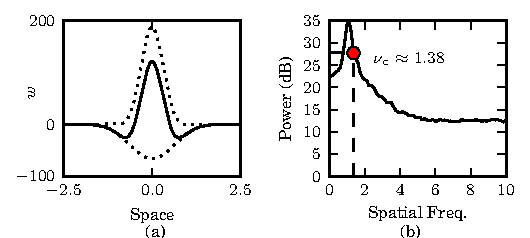
\includegraphics[scale=1]{./Graph/ObservationFreqResponse.pdf}
 \caption{(a) Mexican-hat connectivity kernel. The kernel is a composite of two B-spline
functions (dashed lines), representing local excitation and lateral inhibition. (b) The average (over time) power in dB of the spatial frequency of the observations generated by the kernel in (a). The dashed line shows the cutoff frequency (-3 dB point).}
\label{fig:KernelAndFreqResponse} 
  \end{figure} 
\begin{figure}[!h] 
 \centering
 %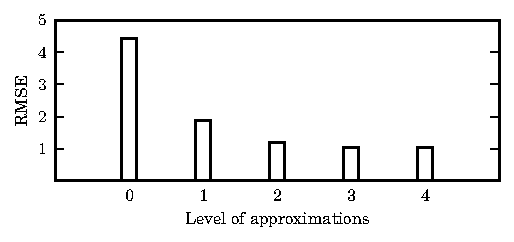
\includegraphics[width=0.5\textwidth]{./Graph/RMSE.pdf}
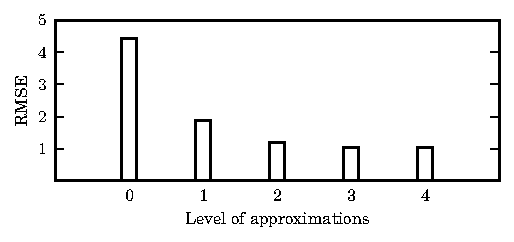
\includegraphics[scale=1]{./Graph/RMSE.pdf}
 \caption{RMSE of the estimated field at different spatial resolution.}
 \label{fig:RMSE}
 \end{figure} 
\begin{figure}[!h] 
 \centering
 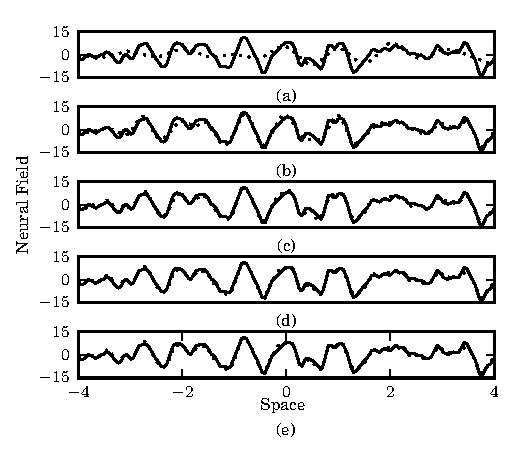
\includegraphics[scale=1]{./Graph/Field.pdf}
 \caption{Spatial field at one time instant for different spatial resolutions, estimated and true fields are shown by dashed and solid lines respectively; (a) $j=0$, $n_x=17$. (b) $j=1$, $n_x=33$. (c) $j=2$, $n_x=65$. (d) $j=3$, $n_x=131$. (e) $j=4$, $n_x=263$.}
 \label{fig:FieldEstimates}
 \end{figure} 
\begin{figure}[!h] 
 \centering
 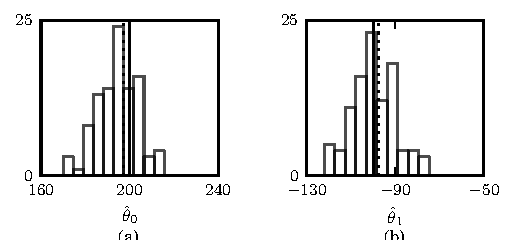
\includegraphics[scale=1]{./Graph/Hist.pdf}
 \caption{Histograms of the parameter estimates over 100 realizations. In each of the subplots
the solid lines show the actual parameter values and the dotted lines show the means of the estimated parameters. Left panel: The histogram of the central excitatory connectivity kernel basis function parameter estimates, $\theta_0$. Right panel: The histogram of the surround inhibition connectivity kernel basis function parameter estimates, $\theta_1$.}
 \label{fig:ParametersHistogram}
 \end{figure} 

\section{Discussion}
Some discussion points
\begin{itemize}
	\item Brief summary of the novel aspects
	\item Discuss how we are improving the previous work
	\item Discuss heterogeneity and time delays (at larger spatial scales) and homogeneity (at smaller scales) 
	\item Discuss assumptions, limitations and future work
\end{itemize}


% In order to estimate the spatial mixing kernel and the spatio-temporal field, the  kernel and the field are decomposed using
% Note that the number of translation operations depends on the spatial range of the data. It follows that the total number of terms in (\ref{1DKernelDecompositionForSimulation}) and (\ref{1DFieldDecompositionForSimulation}) are 8 and 47 respectively. The estimated kernel in \figurename{\ref{fig:SpatialMixingKernelEstimate} } is obtained for the cubic B-spline, with initial scale 0 and maximum scale 1. The EM algorithm is allowed to run for 30 iterations to avoid any issues regarding early stopping, though typically the change in $\parallel \mathbf{A} \parallel_{F}$ falls below $10^{-4} $ after less than 15 iterations. A total number of 500 estimation experiments are performed, where $v_t$ and $w_t$ are re-generated each trial.


%  The performance measure employed here is the Mean Integrated Squared Error (MISE) defined as
% \begin{equation}
%  \mathbf{E}\left[\int_{\mathcal{S}}\left[e\left(s\right) \right]^2ds  \right]
% \label{MISE} 
% \end{equation}
%  where  $e\left(s\right)$ is the error between the unknown function, $f\left( s\right) $ and its estimate, $\hat{f}\left( s\right) $. In this example the original kernel and the field are known and hence the integral in  (\ref{MISE}) can be computed analytically. For spatial mixing kernel we have
% \begin{eqnarray}
%  \lefteqn{\int_{\mathcal{S}}\left[e\left(s\right)\right]^2ds}\nonumber \\  &=\left(\boldsymbol{\theta}-\hat{\boldsymbol{\theta}}\right)^\top\left[ \int_{\mathcal{S}}\boldsymbol\lambda\left(s\right)\boldsymbol\lambda\left(s\right)^\top ds\right] \left(\boldsymbol{\theta}-\hat{\boldsymbol{\theta}}\right)&
% \label{MISEKernel}
% \end{eqnarray}
%   Here, we are particularly interested in assessing the performance improvement as the scale of the details in MRA is increased. Performance based on (\ref{MISEKernel}) at different spatial scales and over 500 trials have been evaluated. The MISE of the model at $j=0$ is 0.024 and reduces to 0.005 when $\psi_{4;1,k}$ terms are also included in the model, in fact estimation performance is improved by a factor of 4.8. The coarsest approximation of the kernel along with its approximation at $j=1$ are illustrated in \figurename{\ref{fig:SpatialMixingKernelEstimate}. It can be seen that the model is able to estimate both slowly and rapidly varying segments of the  kernel with very high accuracy.  Field estimates  at a selection of time instants are shown in \figurename{\ref{fig:1DFieldEstimation}}. It is clearly observed that the coarse and fine features of the original field have been captured accurately over regions where observations are available. Observation locations are generated randomly, as shown in \figurename{ \ref{fig:FieldVariance}}. Assuming the observed field can be fully described by the  decomposed IDE model, the variance of the field can be computed to express the  uncertainty of the estimation, at each point in space and at time $t$ we have 
% \begin{equation}
%  \text{Var}(\hat z_t(s_i))=\boldsymbol\mu^{\top}(s_i) \mathbf P_{t|T}\boldsymbol\mu(s_i)
% \label{eq:FieldVariance}
% \end{equation}
% where $\mathbf P_{t|T} $ is the covariance matrix associated with the  state estimates obtained from the RTS smoother. Variance based on (\ref{eq:FieldVariance}) at each spatial location and at $t=50$ is shown in \figurename{\ref{fig:FieldVariance}}. The uncertainty of the estimation is higher at almost  every spatial location at $j=1$ compared to $j=0$. This is to be expected as there are more wavelet basis functions at higher resolution and hence more associated weights need to be estimated. Peaks in the variance of the field coincide with regions where no observations have been made. Increasing the number of observation locations, or using equally spaced observation locations would reduce the variance of the field estimation.
% \begin{figure}[!h] 
% \centering
% 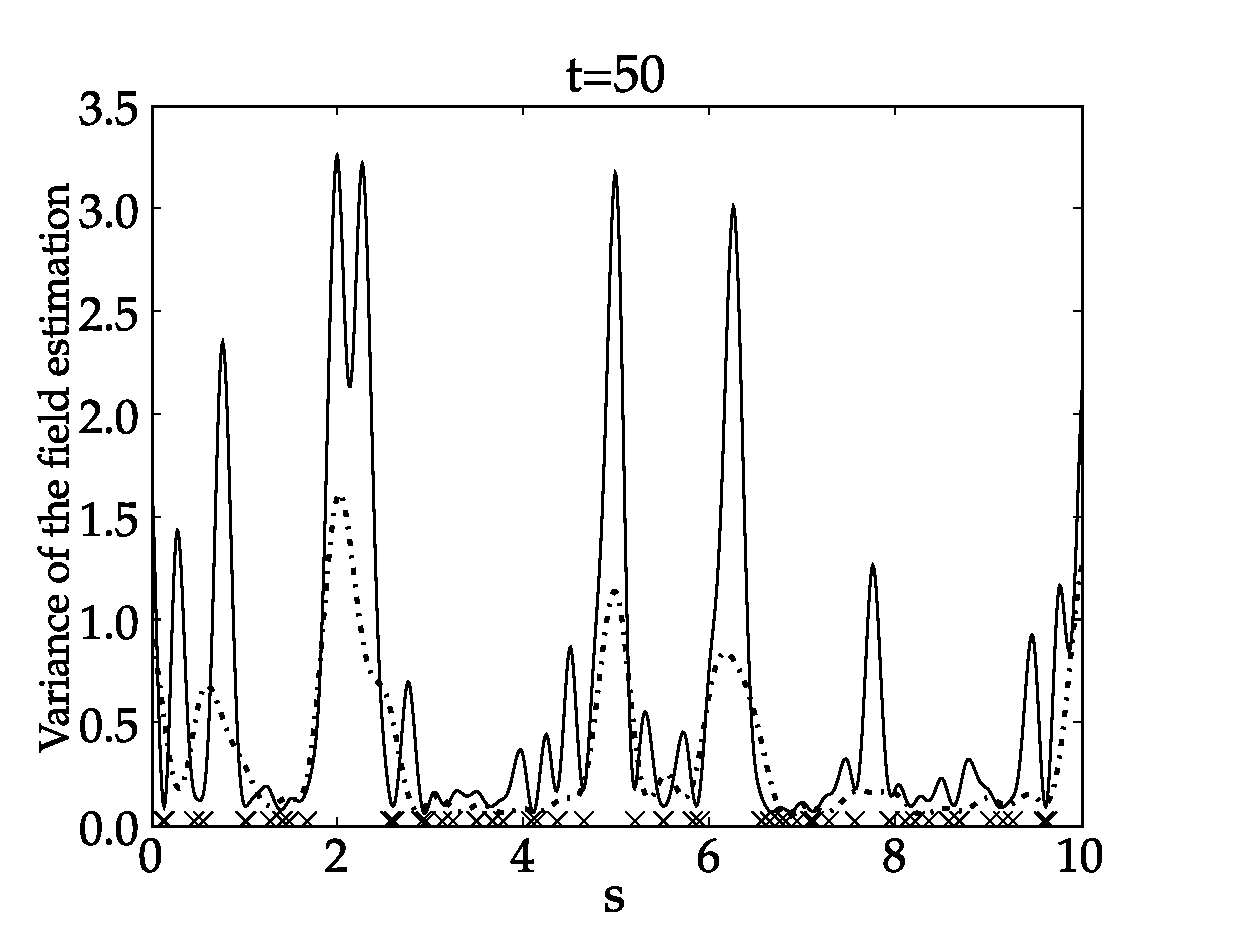
\includegraphics[width=0.5\textwidth]{./Graph/aram4.eps}
% \caption{Variance of the field at each spatial location for $j=0$ (dotted line) and $j=1$ (solid line). The observation locations are described with a cross.}
% \label{fig:FieldVariance}
% \end{figure} 
% \begin{table}[!h]
% \renewcommand{\arraystretch}{1.3}
% \caption {MISE  at particular scale between measured and estimated 2D-field  at a particular time}
% \label{table:ValidationResultField}
% \centering
% \begin{tabular}{cccc}
% \hline \hline
% \multicolumn{2}{r}{Time}&\multicolumn{2}{c}{MISE} \\
% \cline{3-4}
% &&$j=0$&$j=1$ \\ 
% \hline 
% &$5$ &$5.424$&$0.609$ \\
% &$20$ &$5.422$&$0.596$ \\
% &$50$ &$5.519$&$0.626$ \\
% &$100$ &$5.488$&$0.611$ \\
% &$150$ &$5.494$&$0.587$ \\
% \hline \hline
% \end{tabular}
% \end {table}
% \section{Conclusion}
% A multi-resolution approach to modelling spatio-temporal systems has been presented. This model is able to represent continuous-space, discrete-time dynamics at a number of spatial scales simultaneously. This ability greatly extends the class of system which the Integro-Difference Equation can represent.
% 
% 
% By decomposing both the spatial field and the spatial mixing kernel using a wavelet decomposition, it becomes possible to represent small scale details in the field at the same time as large scale details. This is an essential component of any practical spatio-temporal model, without which the model must be artificially separated into global and local modes a-priori.
% 
% 
% The complexity of the model is not affected by the spatial resolution of the observation process, rather it reflects the underlying complexity of the system under study. Therefore, increasing the resolution at which the system is observed does not necessarily increase the complexity of the system identification problem. However the developed algorithm is sensitive to the state dimension, equivalent to the detail represented in the field, and hence intelligent approaches to reduce the number of basis functions is noted as future work. 
% 
% By considering different levels of decomposition, the proposed approach could be used as a method of determining the appropriate scales of decomposition, within a model-selection framework. Combined with an approach to sparsely modelling spatial heterogeneity, such as boundary conditions, this would allow the application of this work to a real-world data set.
% if have a single appendix:
%\appendix[Proof of the Zonklar Equations]
% or
% \appendix  % for no appendix heading
% do not use \section anymore after \appendix, only \section*
% is possibly needed
% use appendices with more than one appendix
% then use \section to start each appendix
% you must declare a \section before using any
% \subsection or using \label (\appendices by itself
% starts a section numbered zero.)
%
% \newtheorem{lemma}{Lemma}
% \begin{lemma}
% Let $N_m\left(s-l_1\right)$ and $N_{m'}\left(s-l_2\right)$ be shifted B-spline functions of order $m$ and $m'$ respectively. Then the inner product of  $N_m\left(s-l_1\right)$  and $N_{m'}\left(s-l_2\right)$ can be calculated by 
% \setlength{\arraycolsep}{0.0em}
% \begin{eqnarray}
% \left\langle N_{m}\left(s-l_{1}\right), N_{m'}\left(s-l_{2}\right)\right\rangle&=&N_{m+m'}\left(m+l_{1}-l_{2}\right) \nonumber \\
% &=&N_{m+m'}\left(m'+l_{2}-l_{1}\right) 
% \end{eqnarray}
% \setlength{\arraycolsep}{5pt}
% \label{lemma:InProduct}
% \end{lemma}
% \begin{IEEEproof}
% The support of $N_m\left(s\right)$ is $\left[ 0,m\right]$ and  is symmetric with respect to $s=\frac{m}{2}$, i.e.
% \begin{equation}
%  N_{m}\left(\frac{m}{2}+s\right)=N_{m}\left(\frac{m}{2}-s\right)
% \label{SymmetrySplieEq}
% \end{equation}
% A direct consequence of (\ref{SymmetrySplieEq}) is 
% \begin{equation}
%  N_{m}\left(s\right)=N_{m}\left(m-s\right)
% \end{equation}
% Therefore
% \setlength{\arraycolsep}{0.0em}
% \begin{IEEEeqnarray}{l}
% \int_{-\infty}^{+\infty}N_{m}\left(s-l_{1}\right)N_{m'}\left(s-l_{2}\right)ds \nonumber \\
% \qquad=\int_{-\infty}^{+\infty}N_{m}\left(m-s+l_{1}\right)N_{m'}\left(s-l_{2}\right)ds \nonumber \\
% \qquad=\int_{-\infty}^{+\infty}N_{m}\left(m+l_{1}-l_{2}-u\right)N_{m'}\left(u\right)du \nonumber \\
% \qquad=\left(N_m \ast N_m'\right) \left(m+l_{1}-l_{2}\right) \nonumber \\
% \qquad=N_{m+m'}\left(m+l_{1}-l_{2}\right) \nonumber \\
% \qquad=N_{m+m'}\left(m'+l_{2}-l_{1}\right) \nonumber
% \end{IEEEeqnarray}
% \setlength{\arraycolsep}{5pt}
% \end{IEEEproof}


%\appendices
%\section{Proof of the First Zonklar Equation}
%Appendix one text goes here.

% you can choose not to have a title for an appendix
% if you want by leaving the argument blank
%\section{}
%Appendix two text goes here.


% use section* for acknowledgement
%\section*{Acknowledgment}

% Can use something like this to put references on a page
% by themselves when using endfloat and the captionsoff option.
\ifCLASSOPTIONcaptionsoff
  \newpage
\fi



% trigger a \newpage just before the given reference
% number - used to balance the columns on the last page
% adjust value as needed - may need to be readjusted if
% the document is modified later
%\IEEEtriggeratref{8}
% The "triggered" command can be changed if desired:
%\IEEEtriggercmd{\enlargethispage{-5in}}

% references section

% can use a bibliography generated by BibTeX as a .bbl file
% BibTeX documentation can be easily obtained at:
% http://www.ctan.org/tex-archive/biblio/bibtex/contrib/doc/
% The IEEEtran BibTeX style support page is at:
% http://www.michaelshell.org/tex/ieeetran/bibtex/
  \newpage
% \bibliographystyle{unsrt} 
% \bibliography{MRAIDE}

\bibliographystyle{IEEEtran}
% argument is your BibTeX string definitions and bibliography database(s)
 \bibliography{IEEEabrv,MRAIDE}

% <OR> manually copy in the resultant .bbl file
% set second argument of \begin to the number of references
% (used to reserve space for the reference number labels box)

% \begin{thebibliography}{1}
% 
% \bibitem{IEEEhowto:kopka}
% H.~Kopka and P.~W. Daly, \emph{A Guide to \LaTeX}, 3rd~ed.\hskip 1em plus
%   0.5em minus 0.4em\relax Harlow, England: Addison-Wesley, 1999.
% 
%  \end{thebibliography}

% biography section
% 
% If you have an EPS/PDF photo (graphicx package needed) extra braces are
% needed around the contents of the optional argument to biography to prevent
% the LaTeX parser from getting confused when it sees the complicated
% \includegraphics command within an optional argument. (You could create
% your own custom macro containing the \includegraphics command to make things
% simpler here.)
%\begin{biography}[{\includegraphics[width=1in,height=1.25in,clip,keepaspectratio]{mshell}}]{Michael Shell}
% or if you just want to reserve a space for a photo:
% \begin{IEEEbiography}{Parham Aram}
% 
%  
% \end{IEEEbiography}
% 
% \begin{IEEEbiography}{Visakan Kadirkamanathan}
% % Biography text here.
% (M’90) received the
% B.A. and Ph.D. degrees in electrical and information
% engineering from the University of Cambridge, U.K.
% He held Research Associate positions at the University
% of Surrey, U.K., and the University of Cambridge,
% U.K., before joining the Department of Automatic
% Control and Systems Engineering, The University
% of Sheffield, U.K., as a Lecturer in 1993, where
% he is currently a Professor of Signal and Information
% Processing and is affiliated to the Centre for Signal
% Processing and Complex Systems. His research interests
% include nonlinear signal processing, system identification, intelligent control
% and fault diagnosis with applications in systems biology, aerospace systems,
% and wireless communication. He has coauthored a book on intelligent control
% and has published more than 120 papers in refereed journals and proceedings of
% international conferences.
% Prof. Kadirkamanathan is the Co-Editor of the International Journal of Systems
% Science and has served as an Associate Editor for the IEEE TRANSACTIONS
% ON NEURAL NETWORKS and the IEEE TRANSACTIONS ON SYSTEMS, MAN, AND
% CYBERNETICS, PART B.
%  \end{IEEEbiography}
% \begin{IEEEbiography}{Michael Dewar}
%  received the M.Eng. degree in
% control systems engineering and the Ph.D. degree
% in systems engineering both from The University of
% Sheffield, U.K., in 2002 and 2007, respectively.
%  He is currently working as
% a Research Associate in the Institute for Adaptive
% and Neural Computation, School of Informatics,
% The University of Edinburgh, U.K. 
% \end{IEEEbiography}

% if you will not have a photo at all:
% \begin{IEEEbiographynophoto}{John Doe}
% Biography text here.
% \end{IEEEbiographynophoto}

% insert where needed to balance the two columns on the last page with
% biographies
%\newpage

% \begin{IEEEbiographynophoto}{Jane Doe}
% Biography text here.
% \end{IEEEbiographynophoto}

% You can push biographies down or up by placing
% a \vfill before or after them. The appropriate
% use of \vfill depends on what kind of text is
% on the last page and whether or not the columns
% are being equalized.

%\vfill

% Can be used to pull up biographies so that the bottom of the last one
% is flush with the other column.
%\enlargethispage{-5in}



% that's all folks
\end{document}


